\cleardoublepage
\chapter{Experimenting with Gaussian processes}
\markboth{Experimenting with Gaussian processes}{Experimenting with Gaussian processes}

In this chapter, we discuss the problem of learning and elucidate what viewpoint will be taken to tackle it. Next, novel results are presented concerning uncertainty estimation in a kernelized setting. Finally, some examples are given to illustrate the general use of the theory.

\section{The control problem}

\section{The building and its HVAC system}

The building considered in this study was a surgery center situated in the São Julião hospital complex, in the city of Campo Grande, MS, Brazil (Figure~\ref{fig.facadeAndRooms}, left). The 51 rooms that compose it are in permanent use and, for information purposes, 528 surgical procedures were carried out in it during August 2021. We were concerned with three thermal zones in its ophthalmology section: two operating rooms (ORs) and one waiting room (WR), all located on the West end of the building (Figure~\ref{fig.facadeAndRooms}, right). Whereas the former rooms are only connected to the waiting room, the latter has a door to the rest of the surgery center. Opaque glass bricks are present in the waiting room as can be seen in the picture, allowing some natural light to enter the space; the operating rooms on the other hand do not feature them, nor do they have any windows. All spaces have exterior walls, but the right-hand side operating room is significantly more affected by direct solar radiation due to the disposition of the nearby trees.

A forced-air HVAC plant is in place to provide the occupants with a suitable indoor climate in accordance with local regulations. A total of seven air-handling units (AHUs) collect outdoor air that is then treated and filtered before being pumped into the several indoor spaces. We had control only over three AHUs, one for each aforementioned thermal zone. A central chiller connected to an external cooling tower provides chilled water to all AHUs, which in turn feature three-way valves to control the flow of water through their cooling coils. The AHU fans are operated always at constant speed, resulting in a constant volumetric flow through the air-ducts and into the zones. As per the regulations, no air recycling is possible and all return air is directly discharged into the atmosphere. As the temperature in Campo Grande is typically high, the HVAC system was conceived to only cool the space, not having the means to provide positive thermal energy (for more details, see Section~\ref{sec.controlProb}).

Two distinct sensor networks were deployed to monitor the HVAC plant and the indoor spaces. Firstly, we will describe the one located in the AHU room. One local controller (LCO)--a National Instruments myRIO--was attached to each air-handling unit, reading all sensors used to monitor the AHUs: supply and return water temperature probes, a water flow meter, an anemometer, as well as an angular position sensor. The LCOs were moreover responsible for running low-level signal processing routines and implementing control actions, i.e., acting on the three-way valve servomotor to change the chilled water flow, hence influencing the supply air temperature. Photos of the AHU room are shown in Figure~\ref{fig.ahuRoom}. Next, in order to measure the indoor temperatures in a flexible way, a wireless network of Z-wave sensors was set up in the operating rooms and waiting room. These were equipped with external temperature probes (Dallas DS18B20) to guarantee fast and precise readings, reporting their measurements periodically to a local computer (LC) that featured a Z-wave transceiver attached to it.


\begin{figure}[!t]
	\centering
	
\includegraphics[width=0.9\linewidth]{../images/chap3_facade.jpg} \\[8pt]
	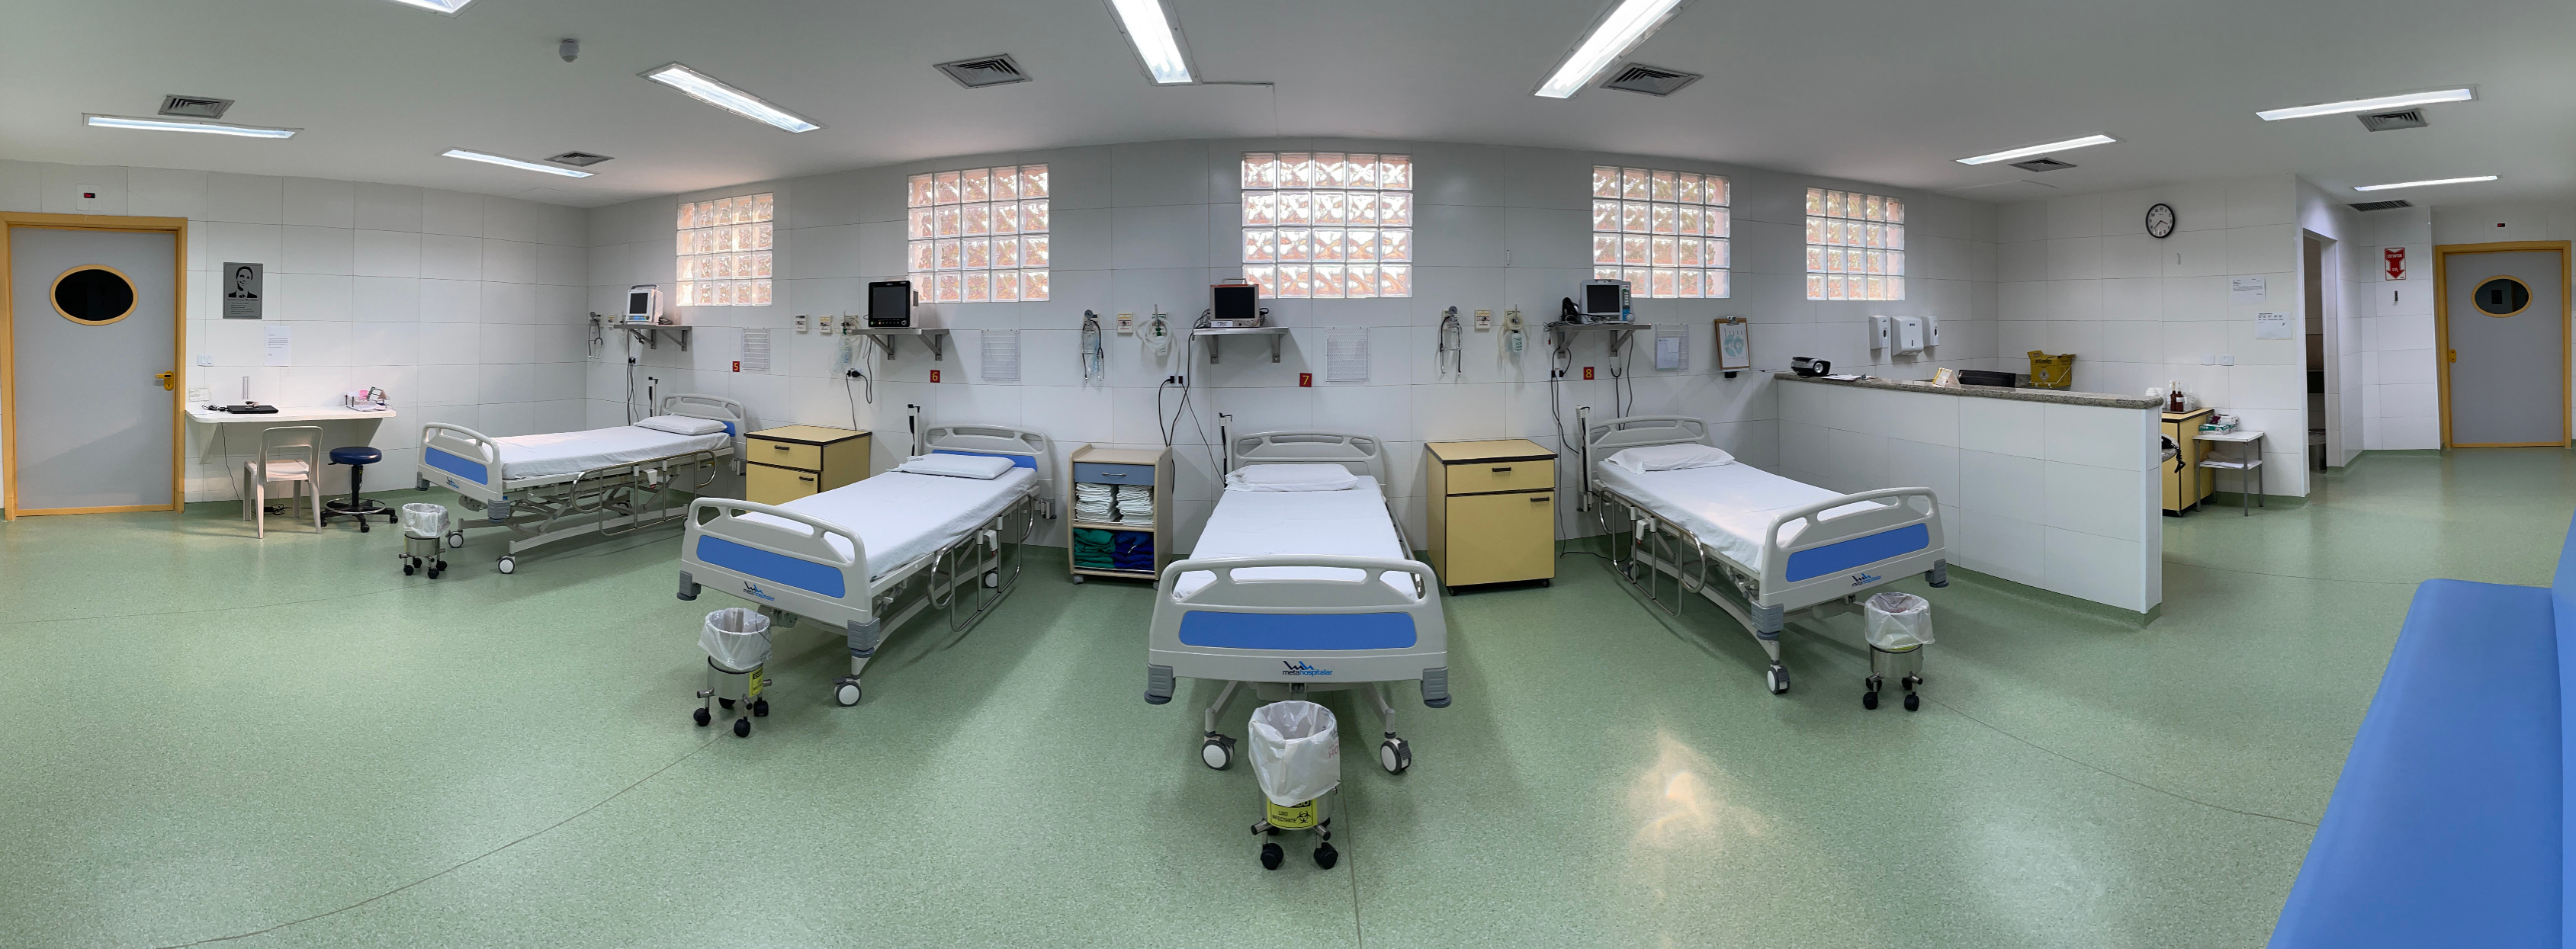
\includegraphics[width=0.9\linewidth]{../images/chap3_rooms.jpg} 
	\caption{Photos of the AHU room depicting the air ducts (top), the supply and return water pipes (top and bottom), and the three-way valve servomotor (bottom).}
	\label{fig.ahuRoom}
\end{figure}

%They periodically report they samples to a 2.66~GHz Mac Mini equipped with a Z-wave USB transceiver that was installed in the waiting room. This local computer (LC) acted as the main computing platform for the project, gathering data from all sources, hosting a local database, and running all the real-time optimization algorithms.
{\tiny }A 3~GHz, 16 GB RAM, core i7 machine was installed in the waiting room, acting as the main computer platform for the project, i.e., the LC. This computer and the AHU LCOs were all connected to a local area network to exchange information, which was done by using the UDP protocol at a rate of approximately 1~Hz. Lastly, a weather station was deployed on site to measure the outdoor temperature and the solar radiation acting on the building with high accuracy. All signals were sampled with a period of two mins and stored into a local time-series database, InfluxDB. A block-diagram of the complete system is depicted in Figure~\ref{fig.blockDiagram}.  

\begin{figure}[!t]
	\centering
	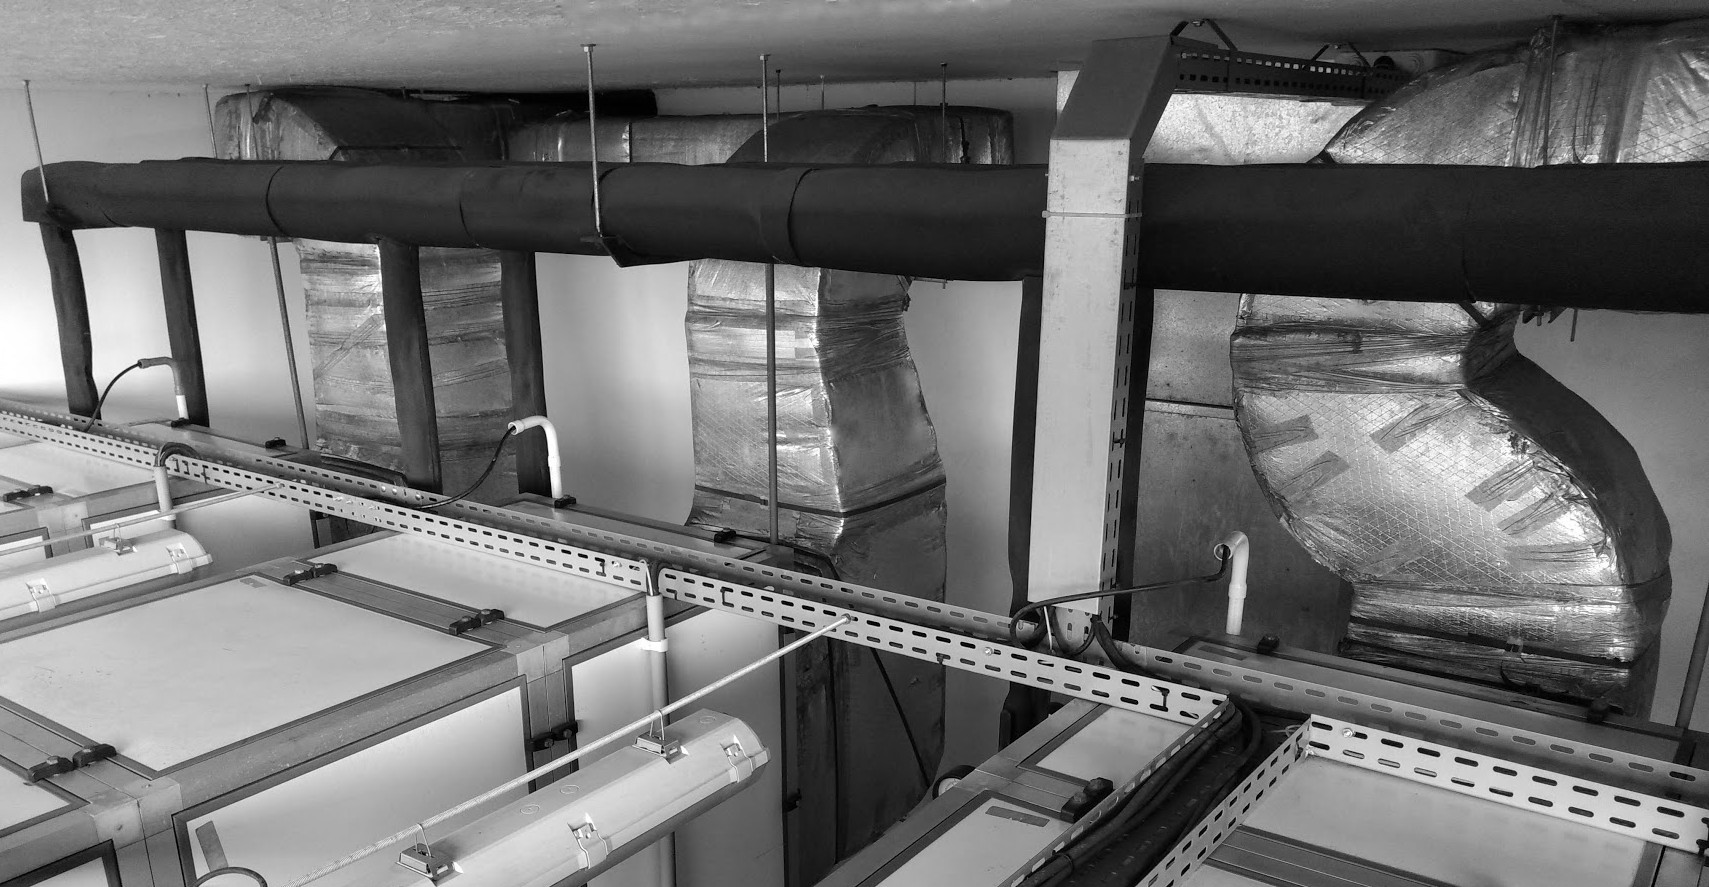
\includegraphics[width=0.75\linewidth]{../images/chap3_ahus_b.jpg} \\[8pt]
	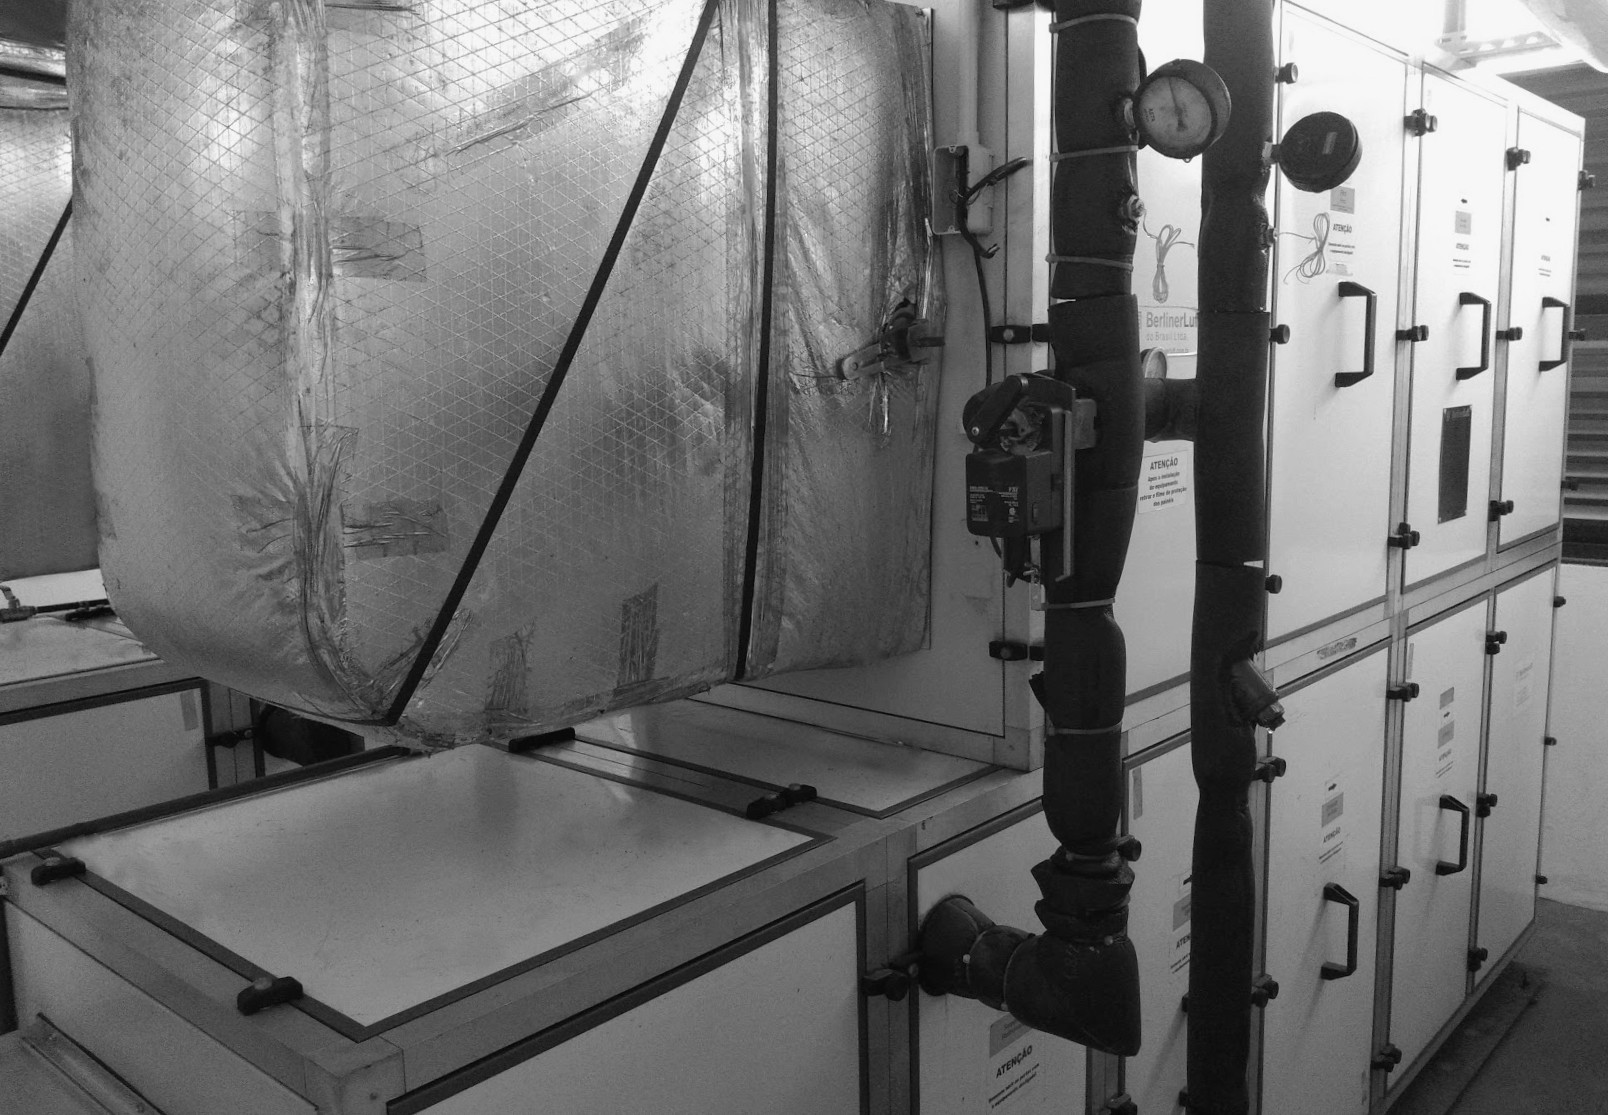
\includegraphics[width=0.75\linewidth]{../images/chap3_ahus_a.jpg} 
	\caption{Photos of the AHU room depicting the air ducts (top), the supply and return water pipes (top and bottom), and the three-way valve servomotor (bottom).}
	\label{fig.ahuRoom}
\end{figure}

\section{The proposed solution}


Given the learned GP models $\mu_i$, $i=1,2,3$ described in \eqref{eq.GPmodels}, a given maximum temperature $T_{\max}$, and our reconstructed electrical power surface, we formulate the following optimization problem to control the valves $\theta_i$ while reducing the chiller energy consumption $E_t$
\begin{subequations}
	\begin{align}
		\min & \quad \sum_{t=0}^{N-1}  \left(E_t + \rho \Delta_t \right) + \rho_N \Delta_N\\
		\text{s.t.}
		& \quad T_{t+1} = \mu(T_t,\theta_t,T_{\text{sup}},T_{\text{out}}) \label{eq.constr1} \\
		& \quad T_t + \beta \, \text{var}^{1/2} (T_t,\theta_t,T_{\text{sup}},T_{\text{out}}) \leq T_\text{max} + \delta_t \label{eq.constr2} \\
		& \quad E_t = Q(T_\text{out},\Theta_t) / \, \text{COP}(Q(T_\text{out},\Theta_t)) \label{eq.constr3} \\
		& \quad \theta_{\text{min}} \leq \theta_t \leq \theta_{\text{max}} \label{eq.constr4} \\
		& \quad \delta_t \geq 0 \label{eq.constr5}
	\end{align}
	\label{eq.optControlProb}%
\end{subequations}
where $\Theta_t = \sum_{i=1}^{3} \theta_{i,t}$ is the sum of all valve positions. The variables $\delta_t$ in \eqref{eq.constr2} are positive slacks introduced to avoid infeasibility. If needed, these can relax the temperature constraint so that the solver can return a viable control plan. Of course, their use is heavily penalized in the objective, where $\Delta_t = \sum_{i=1}^{3} \delta_{i,t}^2$ and $\rho$, $\rho_N$ are large constants, which in our case were respectively set to $100$ and $200$. The temperature constraint \eqref{eq.constr2} also accounts for prediction uncertainty as it includes the standard deviation $\text{var}^{1/2}$. Its use confers on the formulation a risk-aware quality and robustifies the closed-loop operation. The degree of conservativeness is controlled by the constant $\beta$, chosen to be $2$ as in Figure~\ref{fig.trainTestRes}. The prediction horizon was set to $N=12$ steps, which translates to 2 hours. As suggested by our notation, $T_\text{out}$ and $T_\text{sup}$ were kept constant throughout all prediction steps--but updated from one sampling period to the next. Finally, our maximum temperature value was $T_{\max} = 21$ degrees Celsius.

The optimization problem \eqref{eq.optControlProb} was written in \texttt{Python} with the aid of CasADi \cite{casadi}, an automatic-differentiation package that provides gradient information for numerical solvers--in our case, the interior-point method IPOPT. As is customary in predictive control, \eqref{eq.optControlProb} was recursively solved on-line with the most recently available system information, with only the first optimal control action being transmitted to the valves. We underline that the main source of complexity in \eqref{eq.optControlProb} is the presence of the constraints \eqref{eq.constr1} and \eqref{eq.constr2}, which are highly non-linear due the GP mean and variance. Since convexity is absent, multiple local optima might exist, a fact that was indeed verified in practice. By intelligently providing solvers with high-quality initial guesses, this problem can be mostly overcome. Our particular case study relied on initializing the numerical solver with control, temperature, slack and energy trajectories obtained with a virtual PI controller. The intuition was to allow the MPC loop to build on such an initial guess and further optimize operation. For a detailed study on solve times and how the number of GP data-points impacted them, see Appendix~A.


\section{Experimental results}


The previously described Gaussian process-based MPC formulation was deployed on the local computer and used to operate the HVAC system during multiple days in the months of October and November 2021. We report in Figure~\ref{fig.prettyCool} a four-day uninterrupted experiment carried out from November 10 to November 13 that is rather representative of the local internal and external conditions. The plots show the room temperatures and the ``immediate'' uncertainty associated with the GP predictions: $T_\text{unc} = \beta \text{var}^{1/2}$ as employed in the formulation \eqref{eq.constr2}, and evaluated for the next time-step. Both outdoor signals, the temperature and the solar radiation, are also given. The reader is reminded that, although the latter contributes with additional heat gains, it is completely unknown to the controller as explained in Section~\ref{sec.ModelTrainingAndTesting}. We highlight that the curves displayed in the figure were not filtered in any way; the sole manipulation performed with the data was the imputation of the missing temperature entries using linear interpolation. These points, however, accounted for only 43 out of the 1728 indoor temperature values gathered during the four-day experiment.

\begin{figure*}[!t]
	\centering
	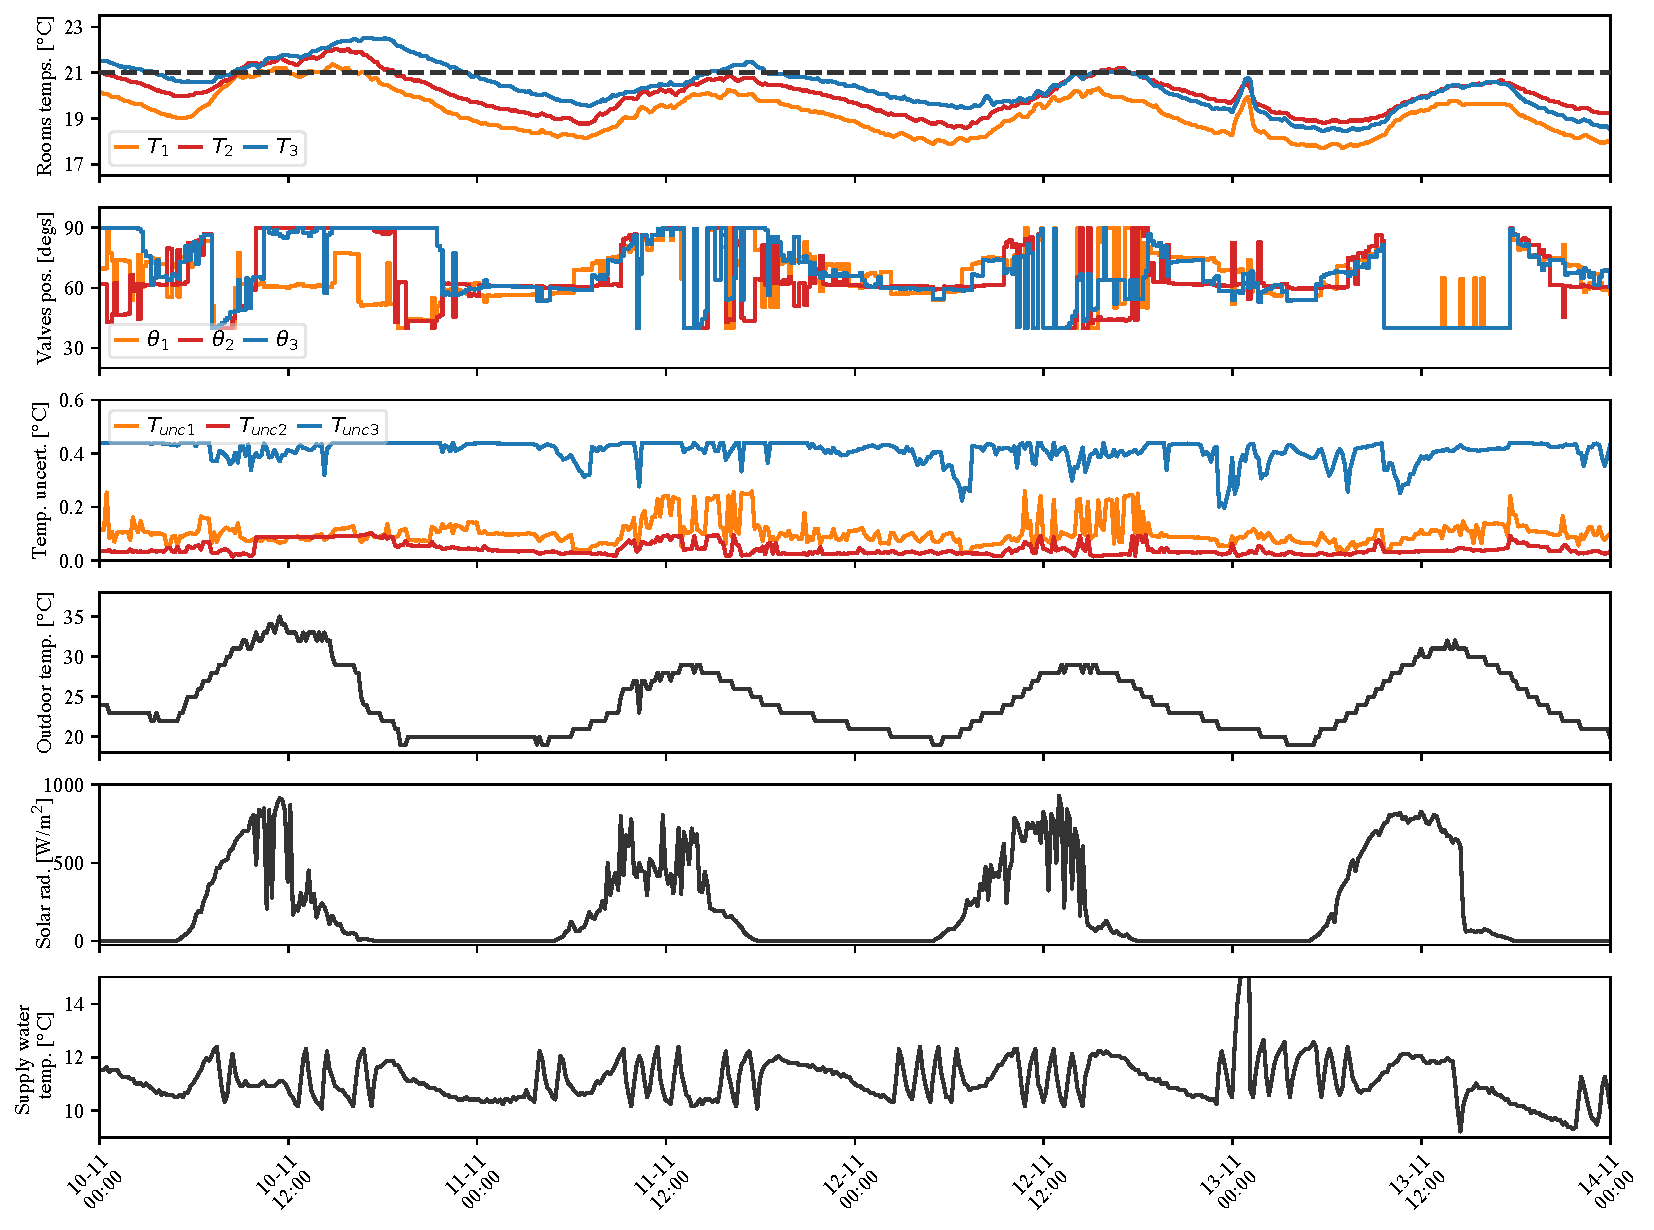
\includegraphics[width=1\linewidth]{../images/chap3_expres.pdf} 
	\caption{MPC experimental results over four days: indoor temperature, valve position and uncertainty estimate associated with each room (top three plots); outdoor temperature, solar radiation and AHUs supply water temperature (bottom three plots). The system was sampled and controlled with a periodicity of 10 minutes.}
	\label{fig.prettyCool}
\end{figure*}

Consider first the day November 10 and note the relatively high internal room temperatures when the experiment started, which were the consequence of a harsh previous day. The MPC controller used some control authority to bring the temperatures below the 21-degree line and then partially closed the valves. After the morning shift started (7 am), even though $\theta_2$ and $\theta_3$ were fully open, $T_2$ and $T_3$ violated the constraints and were only brought below 21 degrees late that evening. High initial conditions along with a peak outdoor temperature of 35 degrees overloaded the cooling system, causing violations of the indoor temperature constraint in two rooms. 

The two days that followed (November 12 and 13) were less warm and, as a result, the MPC controller successfully modulated the valves so as to guarantee constraint satisfaction. It is evident how $\theta_1$, $\theta_2$ and $\theta_3$ assume lower values when $T_\text{out}$ is low, and tend to saturate at their maximum during working hours, which matches our intuition. 

Lastly, we focus on the data from November 13, where one can readily see a sudden peak in the indoor temperatures, being also present in $T_{\text{sup}}$. This was caused by a momentary halt in the water pumps responsible for the chilled water circuit--an event that could be regarded as a fault from a control system perspective. During this period, as there was no water circulation through the AHU cooling coils, there was also no refrigeration and the indoor spaces received warm air since the fans were kept on. As soon as the pumps were again activated, the chiller immediately decreased the supply water temperature and the operation was normalized. During daytime, the indoor climate was kept within the desired limits despite the valves staying saturated at their low values, even at noon. The fact that almost no additional actuation was needed is due to that day being a Saturday, when no operations are scheduled and the three doors present in the environment are minimally opened and closed. This demonstrates how strong the internal heat gains and unmeasured disturbances normally are.

\begin{figure*}[!t]
	\hspace{0pt}
	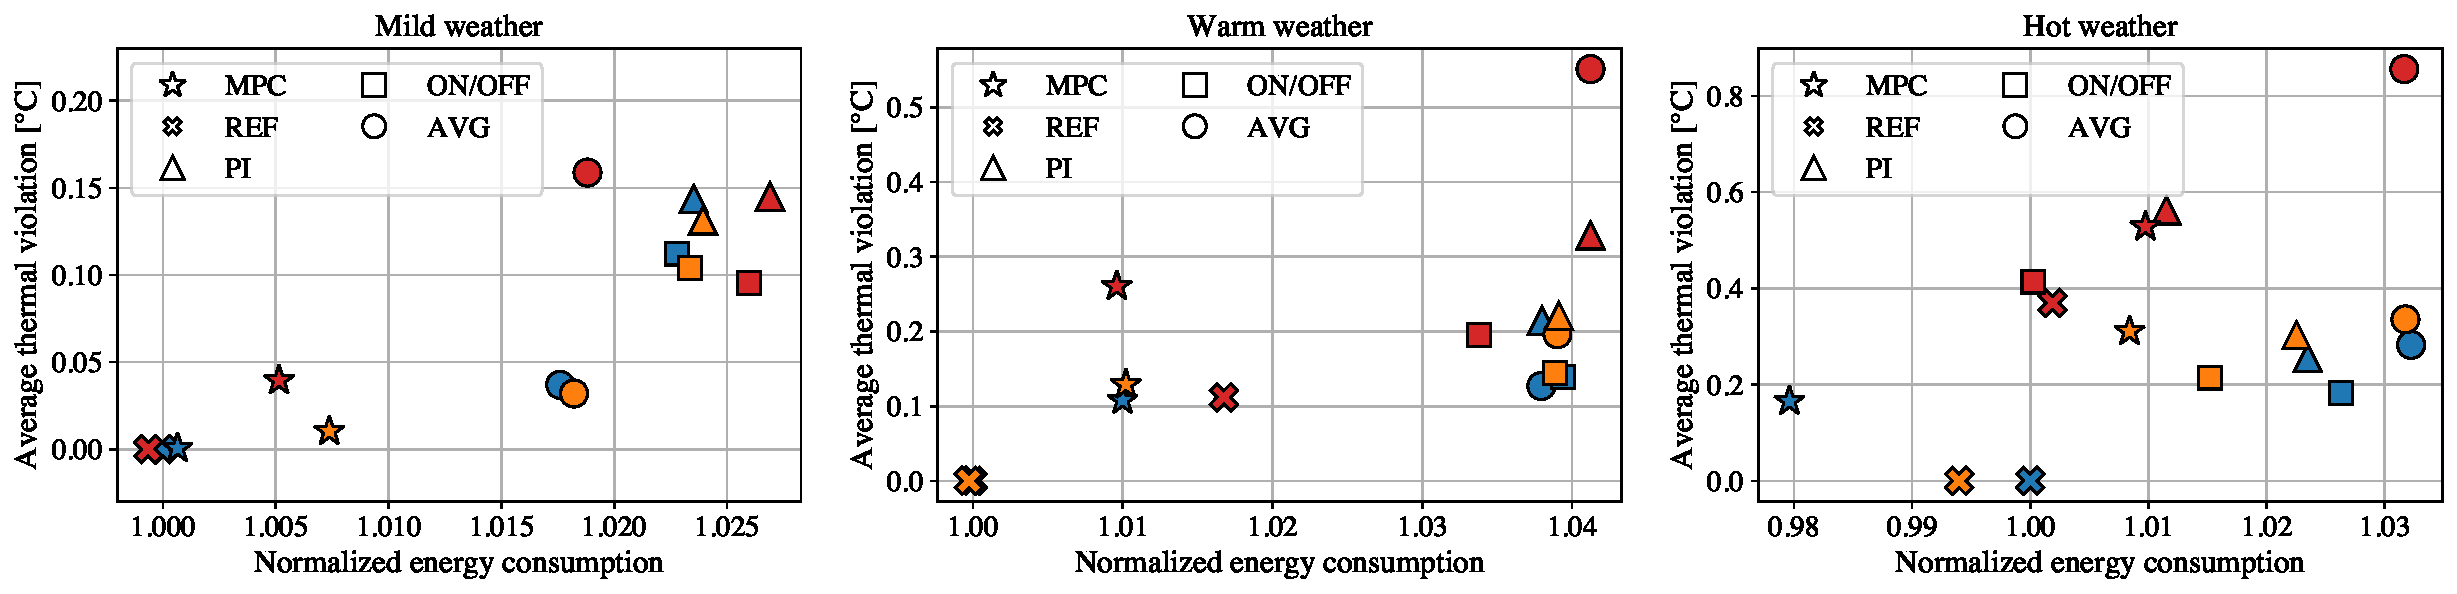
\includegraphics[width=0.95\linewidth]{../images/chap3_simres.pdf} 
	\caption{Simulation results of the normalized energy consumption and thermal performance (average temperature bound violation) of different control strategies. Three weather profiles were considered: mild, warm and hot. The indoor temperatures were initialized at different values according to the color scheme:...} 
	%{\Large \textcolor{color_20}{\textbf{-}}} 17 °C, {\Large \textcolor{color_21}{\textbf{-}}} 19 °C, {\Large \textcolor{color_22}{\textbf{-}}} 21 °C.}
	\label{fig.powerRes}
\end{figure*}

To assess the efficiency gains as well as the thermal performance of the deployed strategy, MPC was compared to alternative algorithms, all subject to exactly the same environmental conditions by means of simulations. We underline that this simulation model was calibrated on data that was \textit{not} included in the GPs training set, thus putting to test the MPC prediction capabilities. The disturbance signals $T_\text{out}$, $T_\text{sup}$ and $R_\text{sol}$ from November 10 were employed, and the indoor temperatures of the three rooms were uniformly initialized at values ranging from $17$ to $21$ degrees Celsius. The outdoor temperature profile was processed to yield three different weather scenarios: hot weather, which was exactly the same $T_\text{out}$ curve seen in Figure~\ref{fig.prettyCool}; warm weather, a $-2$°C shifted version of it, peaking at 33°C around noon; and mild weather, a $-5$°C shifted version of it, peaking at peaking at 30°C. Besides the MPC algorithm \eqref{eq.optControlProb}, the following were also tested:
\begin{itemize}
	\item \red{An MPC controller (herein referred to as REF) with perfect prediction capabilities, perfect disturbance information ($T_\text{out}$ and $T_\text{sup}$)} and a long prediction horizon of five hours.
	\item PI controllers featuring anti-windup schemes and feedforward components to enhance their performance.
	\item Rule-based ON/OFF controllers that set the valves respectively to $\theta_\text{min}$ and $\theta_\text{max}$ if the indoor temperatures were below or above the set-point. 
	\item An average $(\theta_\text{max}-\theta_\text{min})/2$ controller (AVG) whose instantaneous values are selected by sampling the interval $\theta_\text{min}$ to $\theta_\text{max}$ using a uniform distribution.
\end{itemize}

In order to gauge the energy saving potential of the HVAC plant, we executed the REF strategy described above. This algorithm can reach significant efficiency gains while guaranteeing thermal comfort since \red{it exploits a perfect internal model as well as perfect forecasts of the outdoor and supply water temperatures.}

The obtained normalized energy consumption results and average room thermal comfort violations are shown in Figure~\ref{fig.powerRes}. Since the \red{non-linear chiller curves described in Section~\ref{sec:learningChiller} were employed to measure the energy consumption}, the reader is reminded that there is a non-trivial relationship between the weather conditions and indoor temperatures, and the final consumed energy. \red{This aspect is due to the nature of the chiller and not the use of any particular control technique.} As a last note, one specific energy normalization factor was used for each weather scenario shown in Figure~\ref{fig.powerRes} to enhance clarity.

Glancing at the mild and warm weather plots, one notices how the REF and MPC data tended to be close together, and relatively far from the PI, ON/OFF and AVG clusters. Moreover, the REF and MPC points were also mostly to the left side and vertically below the other data given the same indoor temperature conditions--thus confirming their superior performance in terms of energy efficiency and indoor climate regulation. The ON/OFF and PI controllers yielded overall similar numerical results and, surprisingly, were outperformed by the AVG scheme under mild weather and starting indoor temperatures of $17\,$°C and $19\,$°C. AVG nevertheless performed poorly under warm weather and $21\,$°C, and hot weather in general. \red{All in all, the predictive control strategies MPC and REF yielded the best results in the mild and warm weather cases, whereas the separation among them and the other techniques became less evident under hot weather, indicating a less important advantage over classical control.}

By analyzing the horizontal scales and contrasting REF to PI, ON/OFF and AVG, one concludes that this particular HVAC plant could have its efficiency boosted by approximately 2.5\%, 4\% and 5\% respectively in the mild, warm and hot weather scenarios. Notice how, as opposed to studies such as \cite{bunning2020experimental}, these numbers refer to the electrical energy associated with a chiller, and not to a cumulative thermal energy. Moreover, as the hospital was not subject to time-varying electricity prices, the contrast among control strategies was not as broad as for instance the one reported in \cite{joe2022investigation}. The proposed MPC strategy \eqref{eq.optControlProb} attained results close to the aforementioned maximum percentages. Quantitatively, MPC lead to a maximum energy efficiency improvement of 2.29\%, 3.13\% and 4.76\% respectively in mild, warm and hot weather, when compared to the PI and ON/OFF counterparts.
